\documentclass{article}
\usepackage[utf8]{inputenc}
\usepackage[english]{babel}
\usepackage{graphicx}
\usepackage{float}
\usepackage{listings}
\usepackage{hyperref}
\usepackage{amsmath}
\hypersetup{
    colorlinks=true,
    linkcolor=blue,
    filecolor=magenta,      
    urlcolor=cyan,
}
\urlstyle{same}

\title{Manual 4 - 2do Torneo de Programación Competitiva}
\author{Lions R.C.}
\date{Julio 2019}

\begin{document}

\maketitle

\tableofcontents

\begin{figure}[H]
    \centering
    
\includegraphics[width=0.2\paperwidth]{newblack}
\end{figure}

\section{Arreglos multidimensionales}

A veces es conveniente manejar datos como si fueran a estar en una matriz de más de una dimensión, asi que C++ te permite crear arreglos multidimensionales para facilitar este proceso. Casi nunca se requieren más de tres dimensiones para resolver un problema asi que el usuario debe definir previamente cuantas dimensiones tiene su arreglo, además la memoria que se requiere para el arreglo incrementa exponencialmente con cada dimensión.

Para definir un arreglo de dimensión N, se debe escribir el tipo de dato, el nombre del arreglo y N corchetes \textbf{[]}. Si queremos un arreglo de 7 x 3 x 3 enteros, podemos definirlo con \textbf{int miArreglo[7][3][3];}. También se pueden definir los datos iniciales de este arreglo utilizando multiples llaves anidados:

\begin{lstlisting}[language=C++, caption=Asignando valores]
#include <iostream>

using namespace std;

int main() {
    int cuboide[2][3][3] = {{{1, 2, 3}, {4, 5, 6}, {7, 8, 9}},
    {{10, 11, 12}, {13, 14, 15}, {16, 17, 18}}};
}
\end{lstlisting}

\section{Structs}

A veces es frustrante tener que manejar grupos de datos que deben ir juntos debido a que se tienen que crear pares de pares o multiples arreglos. Esto se puede solucionar con los structs, que son parte de la programación orientado a objetos.

Los structs son estructuras que un usuario puede definir para guardar multiples variables bajo un solo "objeto".

Por ejemplo, digamos que trabajas para un banco y quisieras guardar los datos importantes de tus clientes: su nombre, su apellido, su número de tarjeta y la cantidad de dinero que tiene. Si quisieramos guardar estos valores convencionalmente, tendriamos que usar cuatro arreglos o cuatro pares de pares anidados.

Usando structs, podemos definir un struct por cada cliente con estos tipos de datos y crear un solo arreglo o vector de clientes. No se requiere ninguna librería para definir un struct y se puede crear de la siguiente manera:

\begin{lstlisting}[language=C++, caption=Definición de un struct]
#include <iostream>

using namespace std;

struct Cliente {
    string nombre;
    string apellido;
    int tarjeta[16];
    float dinero;
};

int main() {

}
\end{lstlisting}

Como se puede ver, los structs siempre deben ir antes de nuestra función main y deben tener un punto y coma despues de su llave de cierre. Luego dentro de las llaves debe tener una lista de todas las variables que se desean agrupar.

Para crear una instancia de un struct, se debe poner el nombre del struct como el tipo de dato seguido por el nombre especifico de esa instancia:

\begin{lstlisting}[language=C++, caption=Instanciamiento]
#include <iostream>

using namespace std;

struct Cliente {
    string nombre;
    string apellido;
    int tarjeta[16];
    float dinero;
};

int main() {
    Cliente jorge;
    Cliente pablo;
}
\end{lstlisting}

Como se puede observar, se crearon dos clientes, \textbf{jorge} y \textbf{pablo}. Podemos modificar sus datos escribiendo el nombre de cada variable despues de un punto:

\begin{lstlisting}[language=C++, caption=Modificando valores]
#include <iostream>

using namespace std;

struct Cliente {
    string nombre;
    string apellido;
    int tarjeta[16];
    float dinero;
};

int main() {
    Cliente jorge;
    jorge.nombre = "Jorge";
    jorge.apellido = "Velazquez";
    jorge.tarjeta = {0, 1, 2, 3, 4, 5, 6, 7, 8, 9, 0, 1, 2, 3, 4, 5};
    jorge.dinero = 50726.35;
    Cliente pablo;
    pablo.nombre = "Pablo";
    pablo.apellido = "Cesar"
    pablo.tarjeta = {3, 1, 4, 1, 5, 9, 2, 6, 5, 3, 5, 8, 9, 7, 9, 2};
    pablo.dinero = 999999999.9999;
}
\end{lstlisting}

Para simplificar este proceso, es más facil guardar las estructuras en un arreglo o vector:

\begin{lstlisting}[language=C++, caption=Clientes bancarios]
#include <iostream>
#include <vector>

using namespace std;

struct Cliente {
    string nombre;
    string apellido;
    int tarjeta[16];
    float dinero;
};

int main() {
    int numeroDeClientes = 3;
    vector<Cliente> clientes;
    for(int i = 0; i < numeroDeClientes; i++) {
        Cliente nuevo;
        cout << "Nombre del cliente: " << endl;
        cin >> nuevo.nombre;
        cout << "Apellido del cliente: " << endl;
        cin >> nuevo.apellido;
        string tarjeta;
        cout << "Tarjeta del cliente: " << endl;
        cin >> tarjeta;
        for(int i = 0; i < 16; i++) {
            nuevo.tarjeta[i] = tarjeta[i] - '0';
        }
        cout << "Dinero: " << endl;
        cin >> tarjeta;
        clientes.push_back(nuevo);
        cout << "Cliente " << nuevo.nombre << " guardado con exito" << endl;
    }
    cout << clientes.size() << " clientes guardados" << endl;
    for(int i = 0; i < clientes.size(); i++) {
        cout << clientes[i].nombre << endl;
    }
}
\end{lstlisting}
\href{https://repl.it/@Jamesscn/Structs}{Liga al código} \\

El último código guarda 5 clientes en un vector y pide sus datos al usuario. Después, se imprimen los nombres de estos clientes.

\section{Grafos}

Un conjunto de datos con relaciones entre otros datos se puede decir que es un grafo. Cada grafo debe de poder ser dibujado en un plano con los datos encerrados entre circulos y con líneas entre estos datos.

\begin{figure}[H]
    \centering
    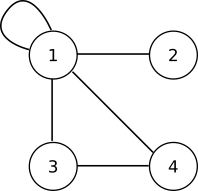
\includegraphics[width=0.15\paperwidth]{grafo}
\end{figure}

En esta imagen, hay cuatro elementos unidos a si mismos. Podemos ver que el 1 tiene enlaces con 1, 2, 3 y 4, el 2 solo tiene un enlace con 1, el 3 tiene enlace con 1 y 4 y el 4 tiene enlace con 1 y 3.

Cada uno de estos elementos puede representar un número, un caracter, un punto en 3D o cualquier cosa que deseas que representan, mientras que cada enlace puede tener un significado importante de ese elemento.

Es importante definir que cada enlace debe consistir en la unión de dos elementos, y estos elementos pueden ser el mismo (por ejemplo el enlace que esta unido al 1 dos veces).

\subsection{Nodos, ramas, hojas y raíces}

Se le conoce como nodo o vertice a cada elemento del grafo y se le conoce como rama, enlace o arista a cada enlace. En el ejemplo de arriba, podemos ver que existen cuatro nodos (1, 2, 3, 4) y cinco ramas (1:1, 1:2, 1:3, 1:4, 3:4).

En casos de ciertos grafos, es conveniente pensar que ciertos nodos son hojas o raices. Abajo hay dos ejemplos de grafos que presentan estos nodos con las hojas marcadas en azul y la raíz marcada en rojo

\begin{figure}[H]
    \centering
    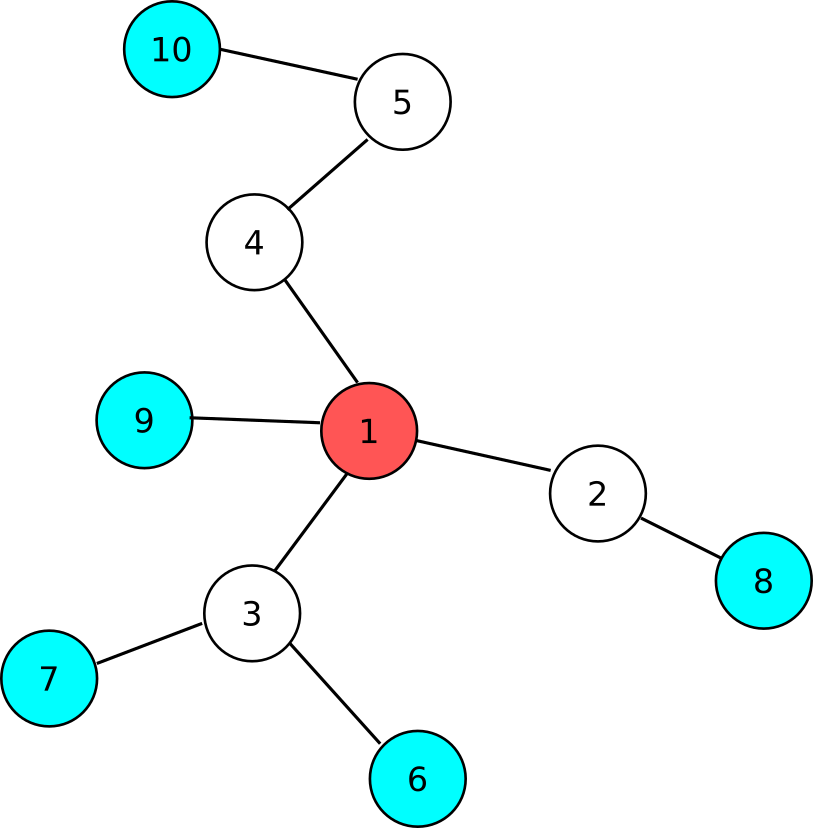
\includegraphics[width=0.25\paperwidth]{expansivo}
\end{figure}

\begin{figure}[H]
    \centering
    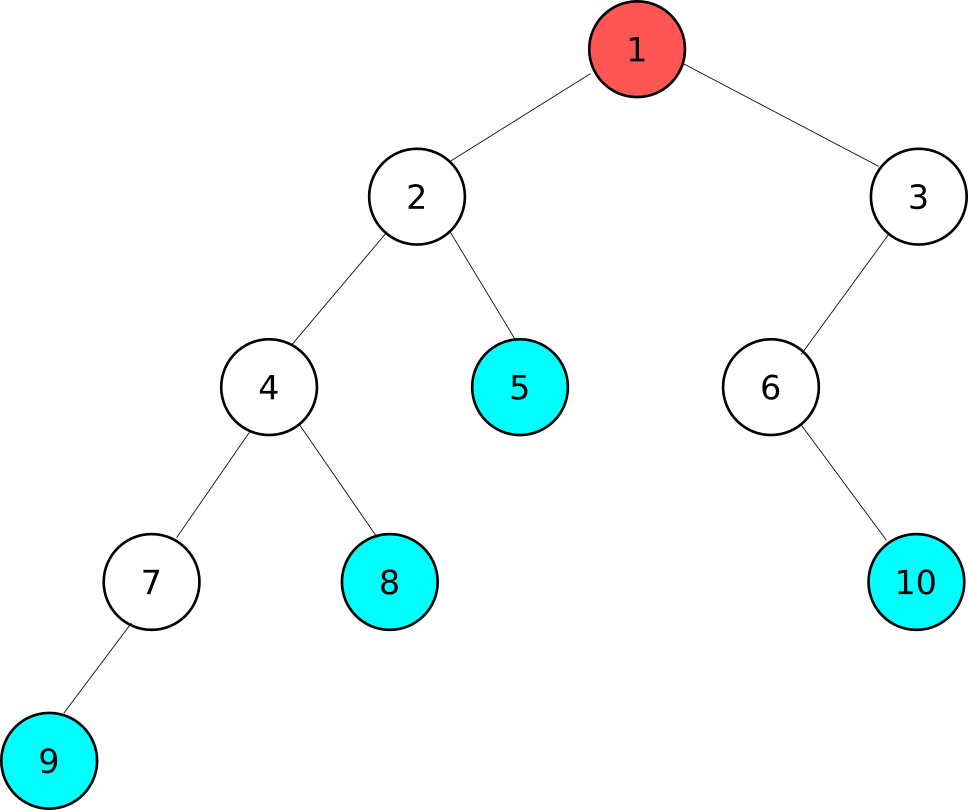
\includegraphics[width=0.3\paperwidth]{arbolbinario}
\end{figure}

Como se puede observar en ambos grafos, existe una raíz o nodo con la mayor cantidad de uniones y que es céntrico a todos los demás nodos, y existen varias hojas que se pueden considerar como nodos que estan en la orilla.

Cada nodo se puede considerar como "hijo" de otro nodo excepto la raíz, y cada nodo se puede considerar como "padre" de otro nodo excepto las hojas. En el primer grafo con la raíz y las hojas señaladas, se puede decir que 2, 3, 4 y 9 son hijos de 1 y que 1 es padre de 2, 3, 4 y 9.

Esta relación de padre y hijo es util será util después para optimizar operaciones relacionados con grafos.

\subsection{Grafos dirigidos y cíclicos}

Hasta ahorita hemos visto grafos no dirigidos, pero también existen grafos dirigidos que tienen ramas de un solo sentido:

\begin{figure}[H]
    \centering
    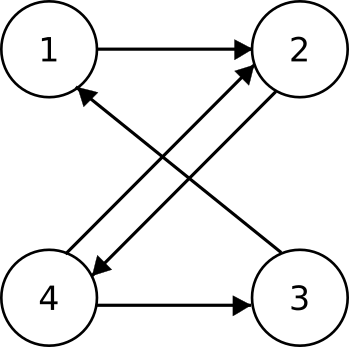
\includegraphics[width=0.15\paperwidth]{dirigido}
\end{figure}

Podemos ver que para llegar desde el nodo 1 al nodo 3 se tiene que pasar por los nodos 2 y 4 porque no hay un camino orientado hacia el nodo 3.

Un ejemplo de un grafo dirigido puede ser el mapa de todas las calles de un pueblo. En el pueblo, puede haber calles de doble sentido o calles de un solo sentido, y se puede representar cada calle como una rama.

Otra propiedad de los grafos ocurre cuando un grafo contiene un ciclo (es decir que puedes llegar a un mismo nodo pasando por ramas distintas en cada salto), entonces ese grafo puede ser considerado como cíclico.

Se puede observar que los dos grafos de la sección \textbf{Nodos, ramas, hojas y raíces} son acíclicos mientras que los otros dos son cíclicos.

\subsection{Grafos con pesos}

Muchas veces es conveniente darle pesos a las ramas de algún grafo para modificar la manera en la que se distribuyen los nodos. Digamos que quieres representar un país con N ciudades o nodos y quisieras saber cual es la mejor ruta de una ciudad a otra.

Para resolver este problema se puede considerar cada rama como una carretera de una ciudad a otra y se le puede poner un peso con la distancia real de esa carretera.

\begin{figure}[H]
    \centering
    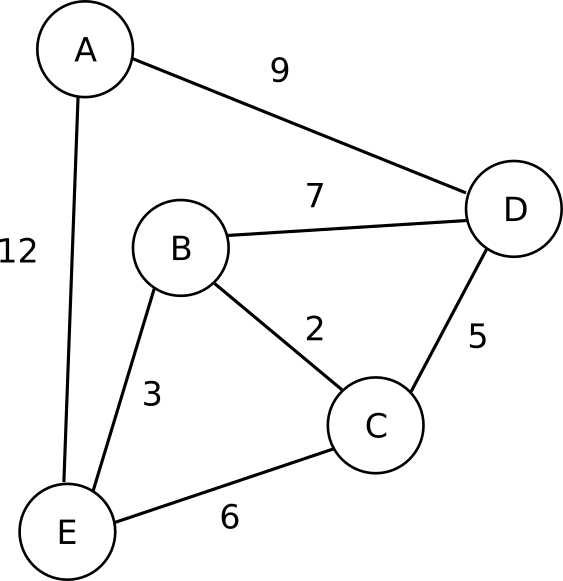
\includegraphics[width=0.2\paperwidth]{ciudades}
\end{figure}

Como se puede observar en el grafo de arriba, hay 5 ciudades (A, B, C, D, E) y varias carreteras con ciertas distancias (en este caso no nos importan las unidades).

Existen muchas posibles maneras de irse de la ciudad E y llegar a la ciudad D, pero solo hay un camino más optimo que los demás. Por ejemplo, podemos tomar el camino E - A - D, pero la suma de las distancias de cada carretera es de 12 + 9 o 21. La mejor opción es el camino de E - B - C - D con una suma total de 3 + 2 + 5 = 10. Se puede ver que a pesar de que se visitaron más nodos se recurrió menos distancia.

La siguiente sección cubre maneras de poder encontrar este camino más óptimo dado cualquier grafo.

\subsection{Arboles binarios}

Un arbol es un tipo de grafo que tiene una raíz en la parte de arriba que crece hacia abajo. Un arbol binario es una especie de arbol donde cada nodo tiene máximo dos hijos, el hijo izquierdo y el hijo derecho.

Este tipo de grafo es popular debido a que se pueden hacer operaciones eficientes sobre sus datos. Se puede implementar este tipo de grafo con un arreglo de tamaño $2^M$ donde M es la profundidad del arbol.

Para guardar un arbol en un arreglo, el primer elemento debe ser la raíz, luego los siguientes 2 elementos deben ser los hijos izquierdo y derecho de la raíz, luego los siguientes 4 elementos deben ser los hijos de esos hijos. Se debe repitir este proceso para llenar el arbol.

En caso de tener un nodo sin un hijo, se puede representar ese hijo con un valor especial.

Si tenemos un nodo en el índice $i$ del arreglo, sabemos que su hijo izquierdo tendría que estar en $2i + 1$ y su hijo derecho estaría en $2i + 2$. También sabemos que el padre de cualquier nodo siempre estará en el índice $\frac{i - 1}{2}$. Esta implementación simplifica la busqueda de nodos.

\begin{figure}[H]
    \centering
    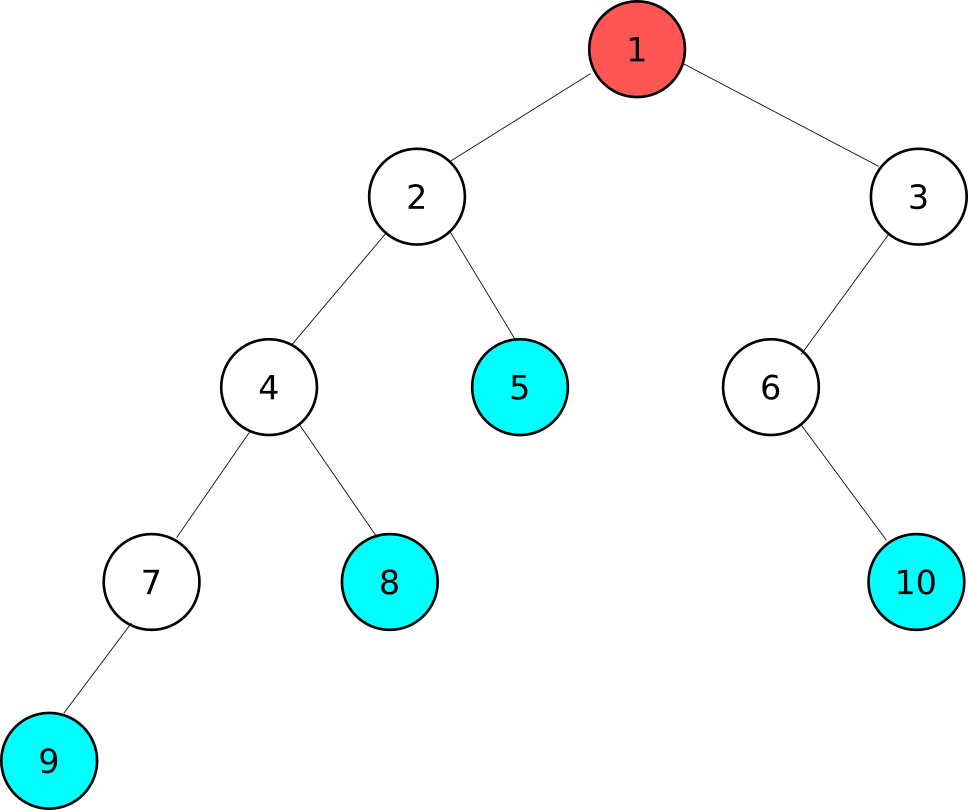
\includegraphics[width=0.3\paperwidth]{arbolbinario}
\end{figure}

Si quisieramos guardar el arbol de arriba en un arreglo de 10 elementos, tendríamos que definir un arreglo de $2^5$ elementos porque su profundidad es de 5. Si suponemos que cada espacio libre tiene valor -1, podemos representar este arbol con el siguiente arreglo: (1, 2, 3, 4, 5, 6, -1, 7, 8, -1, -1, -1, 10, -1, -1, 9).

Si queremos saber el hijo derecho del elemento en el índice 1 (nodo 2), podemos encontrarlo con la formula y se obtiene 2*1 + 2 = 4. Este elemento es el nodo 5 y se puede ver en la gráfica que el nodo 5 sí es el hijo derecho del nodo 2.

Podemos hacer busquedas de nodos con el siguiente código:

\begin{lstlisting}[language=C++, caption=Arbol de binario]
#include <iostream>
#include <vector>

using namespace std;

int main() {
    vector<int> arbol = {1, 2, 3, 4, 5, 6, -1, 7, 8, -1, -1
    -1, 10, -1, -1, 9};
    cout << "Ingresa el numero de un nodo:" << endl;
    int nodoDeInteres;
    cin >> nodoDeInteres;
    int indice = -1;
    for(int i = 0; i < arbol.size(); i++) {
        if(nodoDeInteres == arbol[i]) {
            indice = i;
            break;
        }
    }
    if(indice == -1) {
        cout << "El nodo " << nodoDeInteres << " no es
        miembro de este arbol" << endl;
        return -1;
    }
    if(indice == 0) {
        cout << "Este nodo es la raiz, lo que significa que
        no tiene padre" << endl;
    } else {
        cout << "El padre del nodo " << nodoDeInteres <<
        "es el nodo " << arbol[(indice - 1) / 2] << endl;
    }
    int hijoIzquierdo = 2 * indice + 1;
    int hijoDerecho = 2 * indice + 2;
    if(hijoIzquierdo < arbol.size()) {
        if(arbol[hijoIzquierdo] != -1) {
            cout << "Su hijo izquierdo es el nodo " << arbol
            [hijoIzquierdo] << endl;
        } else {
            cout << "Este nodo no tiene hijo izquierdo"
            << endl;
        }
    } else {
        cout << "Este nodo no tiene hijo izquierdo" << endl;
    }
    if(hijoDerecho < arbol.size()) {
        if(arbol[hijoDerecho] != -1) {
            cout << "Su hijo derecho es el nodo " << arbol
            [hijoDerecho] << endl;
        } else {
            cout << "Este nodo no tiene hijo derecho"
            << endl;
        }
    } else {
        cout << "Este nodo no tiene hijo derecho" << endl;
    }
}
\end{lstlisting}
\href{https://repl.it/@Jamesscn/Arboles-Binarios}{Liga al código}

\subsection{Grafos con arreglos 2D}

Los problemas de grafos más comunes y más faciles tienden a ser esos que ocurren en un plano 2D y que pueden ser representados sobre un arreglo 2D.

Un ejemplo común es pensar en un plano como la vista superficial de un laberinto, y construir un arreglo bidimensional de booleanos donde 1 es una pared u obstaculo y 0 es un camino libre.

Aqui hay un ejemplo donde cada 1 se ha pintado de negro y cada 0 se ha dejado en blanco:

\begin{figure}[H]
    \centering
    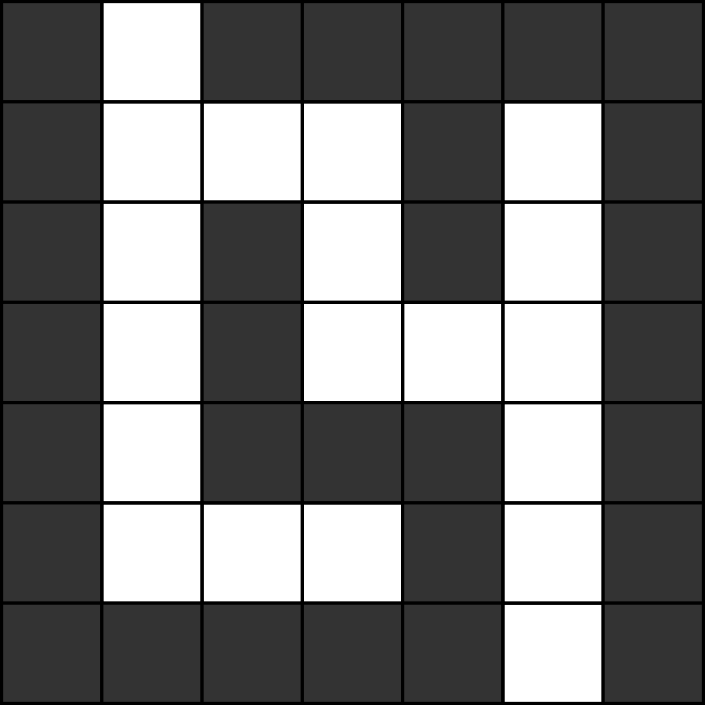
\includegraphics[width=0.2\paperwidth]{grafo2d}
\end{figure}

Si asumimos que somos una persona que esta resolviendo este laberinto y queremos encontrar un camino desde la esquina superior izquierda a la esquina inferior derecha, y solo podemos movernos en cuatro direcciones (arriba, abajo, izquierda o derecha), entonces podemos pensar en este problema como un especie de grafo que podemos resolver.

Ahora hablaremos de como resolver este tipo de problema.

\section{Algoritmos de busqueda}

Los algoritmos de busqueda son métodos especiales de encontrar el camino más corto entre dos nodos de un grafo. Esto tiene muchas aplicaciones, como encontrar la ruta más rapida entre dos ciudades o encontrar la solución a un laberinto.

\subsection{Algoritmos heuristicos o greedy}

Se le denota algoritmo greedy a cualquier tipo de algoritmo que toma la decisión más conveniente en todos los pasos de un conjunto de decisiones.

Podemos demostrar este concepto facilmente con el siguiente laberinto:

\begin{figure}[H]
    \centering
    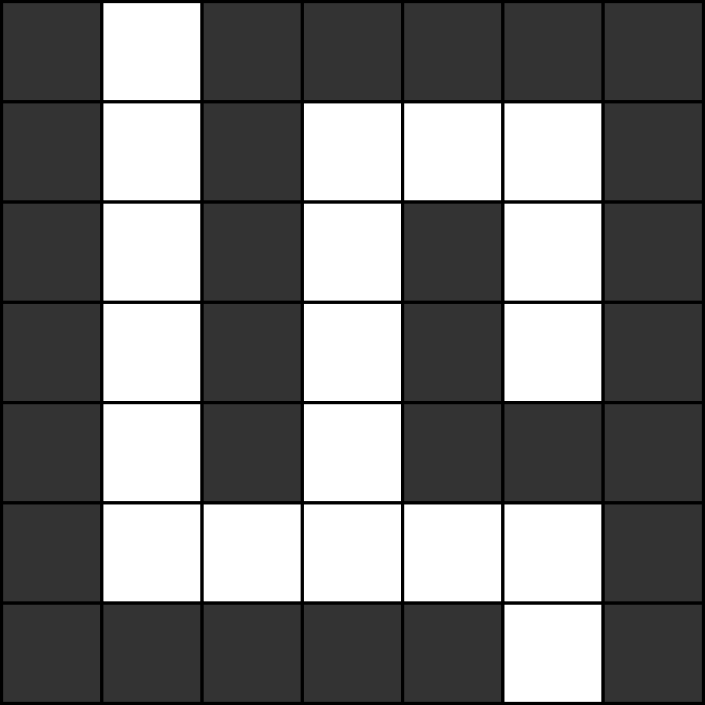
\includegraphics[width=0.2\paperwidth]{greedy}
\end{figure}

Como sabemos que la salida del laberinto siempre estará a nuestra derecha y hacia abajo, entonces un algoritmo greedy nos dirá que siempre debemos mover en una de estas dos direcciones dependiendo de donde estemos.

Primero iniciamos en el primer espacio y solo podemos movernos abajo asi que tomamos esa ruta, luego en el segundo espacio podemos movernos para arriba denuevo o abajo. Decidimos movernos para abajo porque sabemos que la salida está más abajo.

Seguimos esto hasta llegar a la esquina inferior izquierda, y entonces nos empezamos a mover hacia la derecha en lugar de arriba o denuevo a la izquierda porque sabemos que la meta sigue estando a la derecha.

Podemos hacer un programa que prioritiza moverse hacia abajo cuando la meta esta más para abajo que a la izquierda y que prioritiza moverse más para la derecha en caso contrario.

\begin{lstlisting}[language=C++, caption=Camino greedy]
#include <iostream>
#include <utility>

using namespace std;

int main() {
    bool mapa[][7] = {
        {1, 0, 1, 1, 1, 1, 1},
        {1, 0, 1, 0, 0, 0, 1},
        {1, 0, 1, 0, 1, 0, 1},
        {1, 0, 1, 0, 1, 0, 1},
        {1, 0, 1, 0, 1, 1, 1},
        {1, 0, 0, 0, 0, 0, 1},
        {1, 1, 1, 1, 1, 0, 1}};
    pair<int, int> puntoActual = make_pair(1, 0);
    pair<int, int> puntoFinal = make_pair(5, 6);
    int iteracion = 0;
    while(puntoActual.first != puntoFinal.first || puntoActual.second != puntoFinal.second) {
        int x = puntoActual.first;
        int y = puntoActual.second;
        int distanciaX = puntoFinal.first - x;
        int distanciaY = puntoFinal.second - y;
        if(distanciaX > distanciaY) {
            if(mapa[y][x + 1] == 0) {
                puntoActual = make_pair(x + 1, y);
            } else if (mapa[y + 1][x] == 0) {
                puntoActual = make_pair(x, y + 1);
            } else {
                cout << "No se pudo llegar a la meta" << endl;
                return 0;
            }
        } else {
            if(mapa[y + 1][x] == 0) {
                puntoActual = make_pair(x, y + 1);
            } else if (mapa[y][x + 1] == 0) {
                puntoActual = make_pair(x + 1, y);
            } else {
                cout << "No se pudo llegar a la meta" << endl;
                return 0;
            }
        }
        cout << "Iteracion #" << iteracion << endl;
        for(int j = 0; j < 7; j++) {
            for(int i = 0; i < 7; i++) {
                if(i == puntoActual.first && j == puntoActual.second) {
                    cout << "x";
                } else if (mapa[j][i] == 1) {
                    cout << "#";
                } else {
                    cout << " ";
                }
            }
            cout << endl;
        }
        cout << endl;
        iteracion++;
    }
}
\end{lstlisting}
\href{https://repl.it/@Jamesscn/Algoritmos-Greedy}{Liga al código}

Si corremos el código, podemos ver que se encuentra una solución señalada en la grafica de abajo en azúl:

\begin{figure}[H]
    \centering
    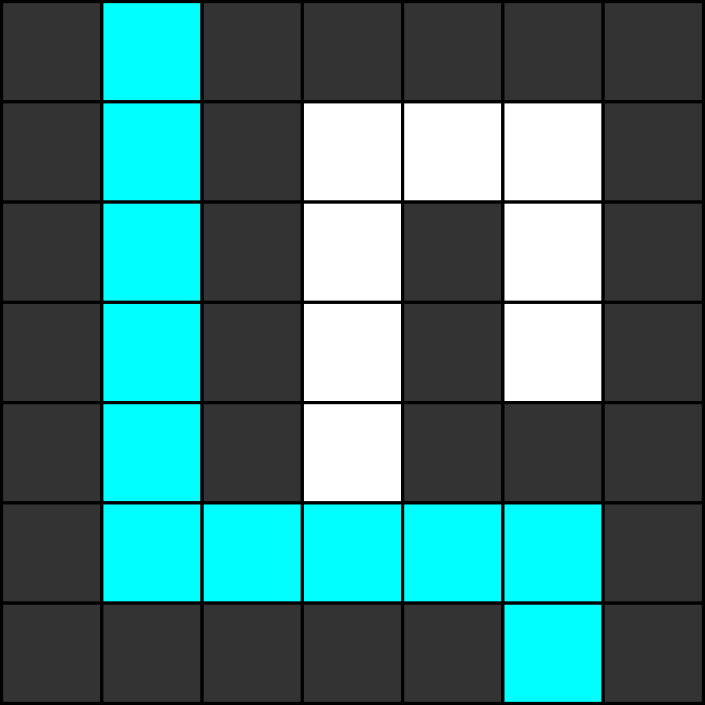
\includegraphics[width=0.2\paperwidth]{greedybueno}
\end{figure}

Pero existen varias desventajas con los algoritmos greedy, particularmente cuando hay caminos que no van a ningun lado. Si hacemos una pequeña modificación al mapa, podemos ver que el algoritmo se atora y no llega a la meta:

\begin{figure}[H]
    \centering
    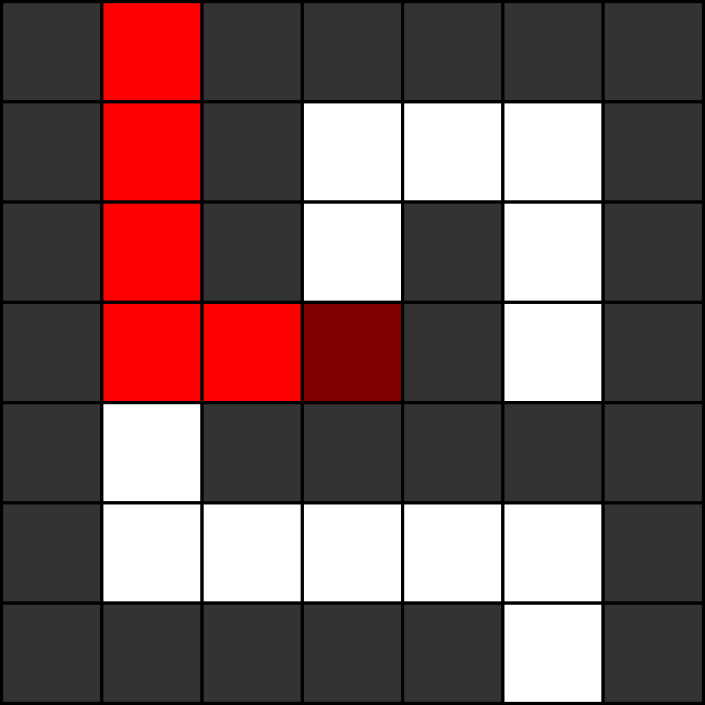
\includegraphics[width=0.2\paperwidth]{greedymalo}
\end{figure}

Esto es porque cuando el algoritmo llegó al cuarto espacio tuvo una decisión de moverse hacia abajo o hacia la derecha. Como el algoritmo piensa que es mejor irse moviendo a la derecha porque la meta esta más a la derecha que abajo, toma un camino falso y se atora.

Se debe observar que en este caso no lo hemos programado para que siga moviendose en caso de haber pared abajo y a la derecha. Esto es porque podría atorarse en un ciclo infinito donde parece que se esta avanzando a la meta pero nunca llega.

Este concepto de heuristica donde se sigue el "instinto" de programa es bueno en ciertos casos, pero no se debe tomar puras decisiones basados en instinto.

\subsection{Busqueda en anchura}

\subsection{Busqueda en profundidad}

\subsection{Algoritmo de Dijsktra}

\subsection{A*}

\section{Punteros}

\end{document}